% Esempio per lo stile supsi
\documentclass[twoside]{supsistudent} 
\usepackage{float}
\usepackage{caption}
\usepackage{listings}

% per settare noindent
\setlength{\parindent}{0pt}


% Crea un capitolo senza numerazione che pero` appare nell'indice %
\newcommand{\problemchapter}[1]{%
\chapter*{#1}%
\addcontentsline{toc}{chapter}{#1}%
\markboth{#1}{#1}
}

% Numerazione delle appendici secondo norma
\addto\appendix{
\renewcommand{\thesection}{\Alph{chapter}.\arabic{section}}
\renewcommand{\thesubsection}{\thesection.\arabic{subsection}}}

\setcounter{secnumdepth}{5} 	%per avere più livelli nei titoli
\setcounter{tocdepth}{5}		%per avere più livelli nell'indice


\titolo{Nuovo algoritmo fotogrammetria - Azienda esterna REX SA}
\studente{Terzi Edoardo}
\relatore{Mattei Yari}
\correlatore{-}
\committente{REX SA}
\corso{Ingegneria informatica (TP)}
\modulo{C10051 Progetto di diploma}
\anno{2019}



\begin{document}

\pagenumbering{alph}
\maketitle
\onehalfspacing
\frontmatter

\pagenumbering{roman}
\tableofcontents
% \listoffigures
% \listoftables	

\mainmatter % suddivide in capitolo 1,2,3 ecc.
\pagenumbering{arabic}
\setcounter{page}{1}

\problemchapter{Abstract}
\section{Italiano}
Questo progetto nasce dalla necessità dell'azienda REX di Mendrisio di creare un sistema
per la progettazione di una passerella posta fra i binari di un passo ferroviario. L'azienda
in questine si occupa della produzione, della progettazione e della vendita di molteplici 
articoli tecnici tra i quali le passerelle. \\

Inizialmente il sistema, costituito da una piattaforma WEB, si occupava di ricevere in input un file DXF realizzato da un geometra 
dell'azienda. Questo file doveva contenere le rilevazioni del geometra, il calcolo delle griglie che costiutiscono la passerella e 
il disegno di queste. Infine la piattaforma generava un documento PDF contenente le istruzioni e il numero di pezzi per il montaggio della passerella.
Inoltre era possibile gestire i clieniti e gli ordini effettuati mediante la piattaforma. \\

Attualmente, in seguito a un progetto di semestre svloto da due studenti della SUPSI, la piattaforma è migliorata mantenendo sempre 
l'aspetto relativo alla gestione degli ordini, dei clienti e del PDF ma è stato alleggerito il lavoro del geometra. Quest'ultimo ora deve inserire 
nel file DXF solamente le misure effettuate e non deve calcolare a mano le griglie necessarie alla costruzione della passerella. \\

L'obiettivo di questo progetto di diploma è quello di rendere ancora più semplice ed automatico l'utilizzo dell'intero sistema mediante l'utilizzo 
di tecniche di processamento dell'immagine. In particolare si vuole realizzare un algoritmo che sia in grado di rilevare le misure necessarie alla costruzione
delle griglie che compongono la passerella partendo da una o più foto della scena, quindi del passo ferroviario dove si vuole fare il lavoro di installazione. \\
\pagebreak
\section{Inglese}
This project stems from the need of the REX company in Mendrisio to create a system
for the design of a footbridge between the tracks of a railway pass. The company
in questine it deals with the production, design and sale of multiple
technical articles including the catwalks. \\

Initially the system, consisting of a WEB platform, took care of receiving a DXF file made by a surveyor
company. This file had to contain the surveyor's data, the calculation of the grids that make up the catwalk e
the design of these. Finally the platform generated a PDF document containing the instructions and the number of pieces for the assembly of the gangway.
It was also possible to manage the customers and the orders placed through the platform. \\

Currently, following a semester project carried out by two SUPSI students, the platform has improved and always maintained
the aspect related to the management of orders, customers and PDF but the surveyor's work was lightened. The latter must now insert
in the DXF file only the measurements made and must not calculate by hand the necessary grids for the construction of the gangway. \\

The goal of this diploma project is to make the use of the entire system even easier and more automatic by using it
of image processing techniques. In particular we want to create an algorithm that is able to detect the measures necessary for construction
of the grids that make up the walkway starting from one or more photos of the scene, then of the railway pitch where you want to do the installation work. \\
\chapter{Introduzione}
\section{Descrizione}
Rex SA è una società manifatturiera: uno dei molti prodotti commercializzati con il proprio marchio è relativo alla
produzione di passaggi di servizio ferroviari in resina per l’attraversamento nelle stazioni ferroviarie e per uscite di
sicurezza nelle gallerie di treno o metropolitana, articoli commercializzati con il marchio SWISSCROSS GFK.
La sfida del progetto risiede nell’implementazione di un sistema capace di creare e visualizzare in modalità aumentata
(sopra una fotografia) un modello virtuale di un passaggio GFK partendo da un'immagine e attivando automaticamente i
processi di produzione, consegna, installazione e, in seguito, di manutenzione del prodotto.
Grazie alla soluzione proposta, REX sarà in grado rafforzare la propria posizione sul mercato svizzero e modificare il
proprio modello di business per iniziare una vendita di servizi digitali a livello internazionale.
Con il progetto si vuole incrementare la competitività dell’azienda delegando al cliente la progettazione e la visione virtuale
del risultato finale in modalità “self-service” prima ancora di confermare l’ordine tramite la piattaforma cloud,
automatizzando quindi ordinazione, produzione e delivery in un vero e proprio processo di Industria 4.0.

\section{Obiettivi}
L'obiettivo principale è quello di sviluppare un algoritmo in grado di sfruttare le metriche conosciute (scarto binari e modelli
3D di binari, traversine e viterie) per ricavare una matrice omografica tramite la quale calcolare il modello completo di una passerella
sulla base di una immagine. Allineamento e sovrapposizione dei modelli generati da più immagini verranno realizzati sfruttando appositi marcatori
posizionati sul terreno. Sintetizzando l'obiettivo di questo algoritmo è quello di permettere l'estrazione dei punti caratteristici da 
un immagine (features) necessari al calcolo della forma e delle misure di una passerella GFK.

\section{Compiti}
Il compito principale risiede nella creazione quindi di un algoritmo in grado di elaborare un immagine fotografica e ricavarne la relativa matrice omografa.
Tramite questa matrice si potrà "raddrizzare" l'immmagine e quindi calcolare le dimensioni reali del passaggio pedonale
che dovrà quindi essere visualizzato in modalità "realtà aumentata" sopra la fotografia.

\chapter{Pianificazione}
\section{Svlogimento del lavoro}

\begin{figure}[H]
  \center
  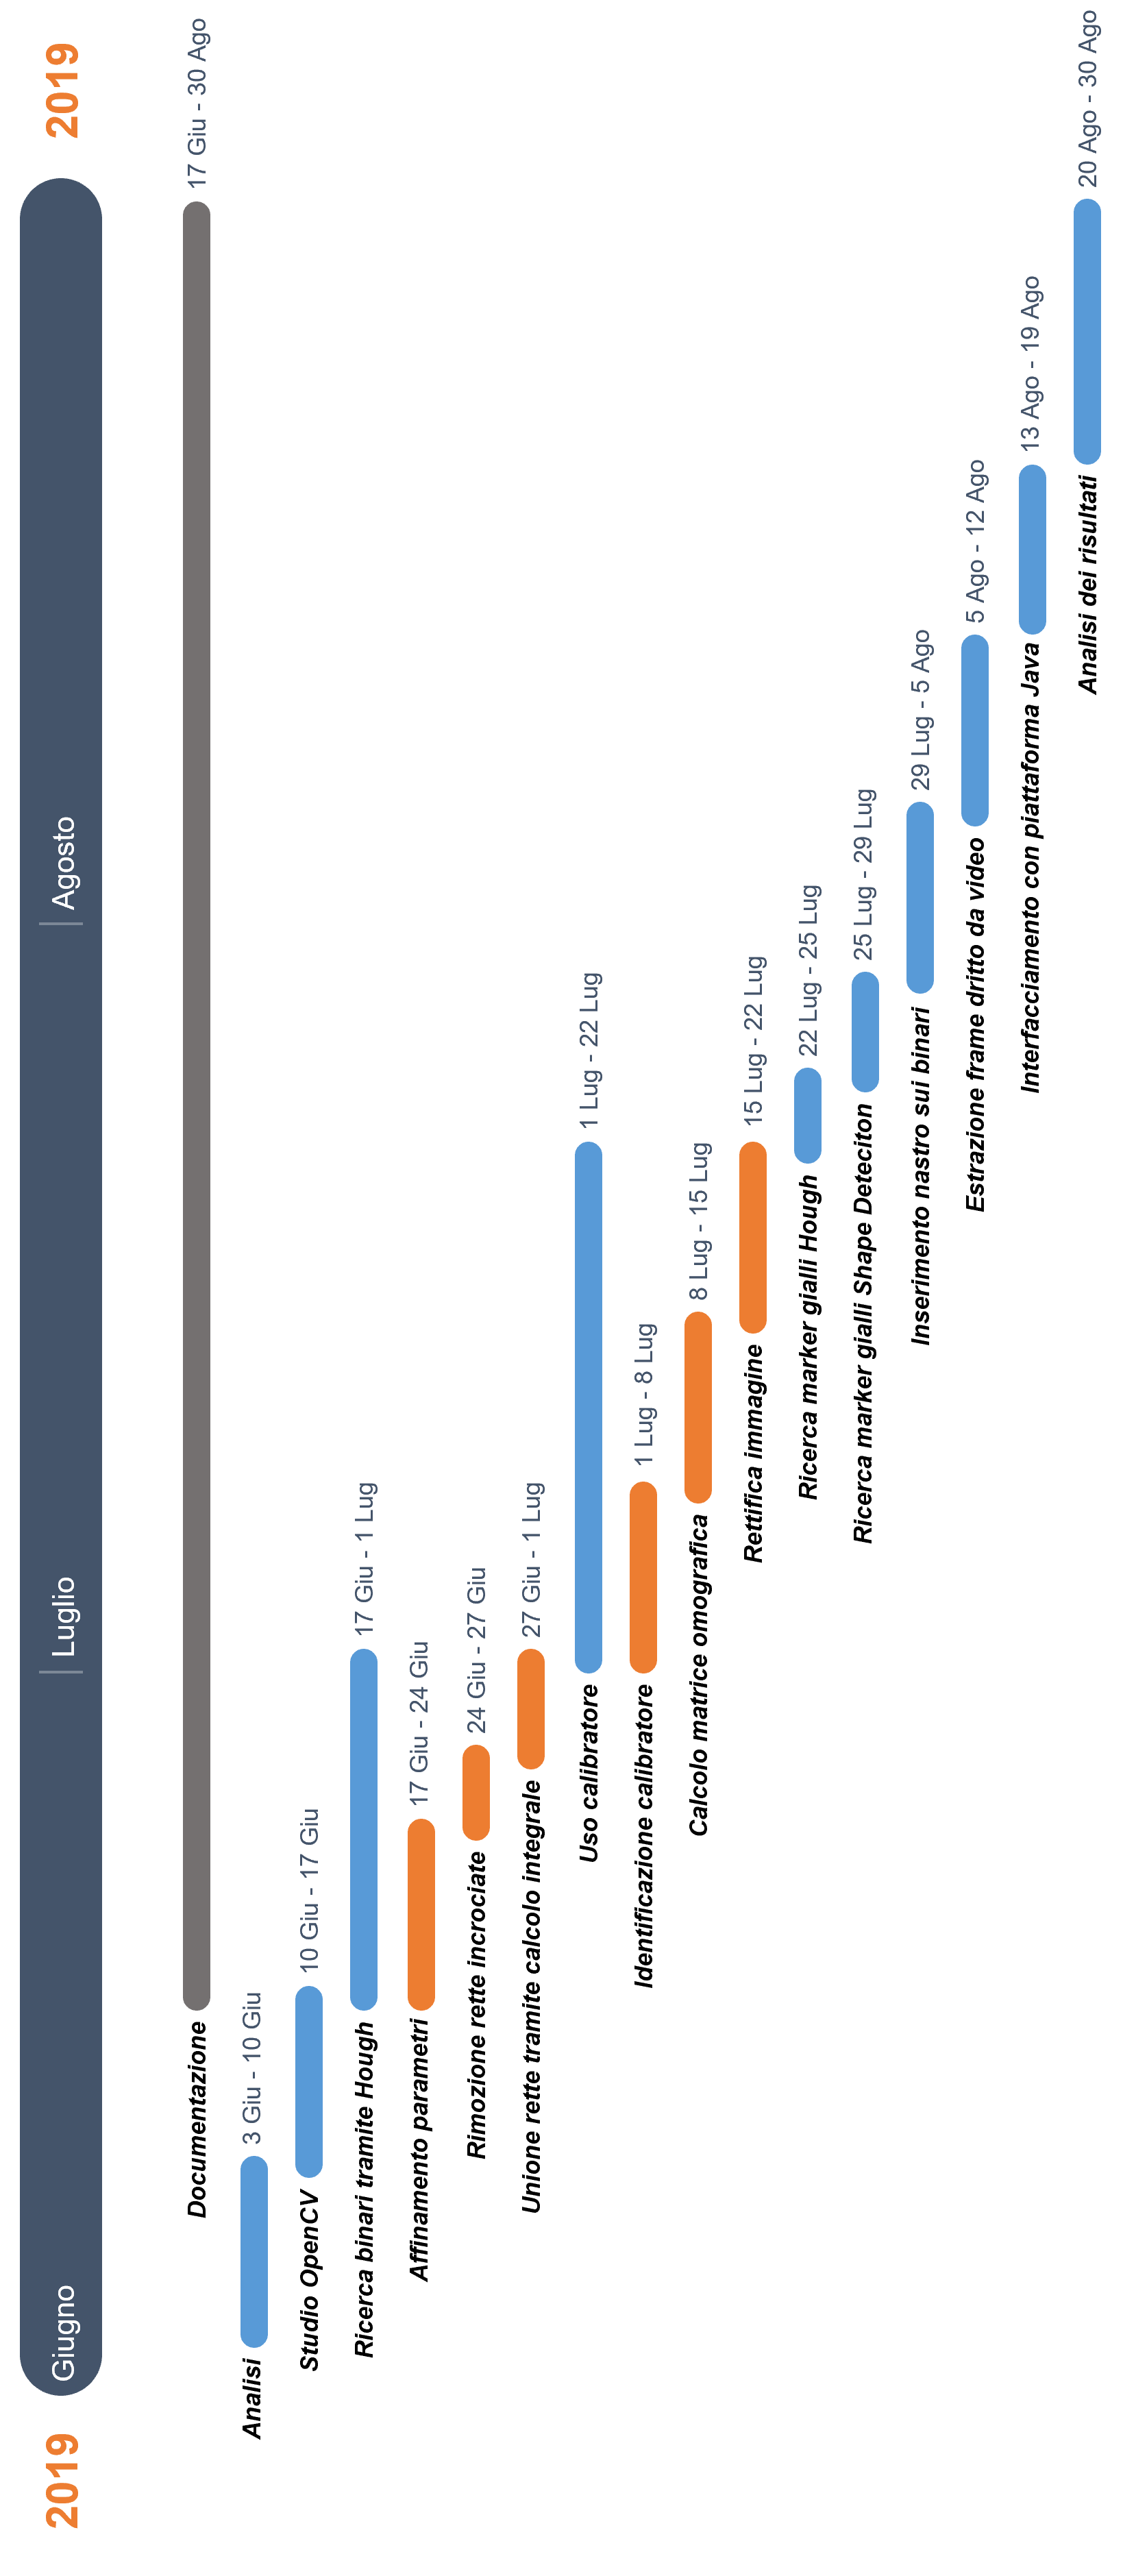
\includegraphics[scale=0.35]{images/Timeline.png}
  \caption{Diagramma di Gantt}
\end{figure}

\chapter{Analisi}
\section{Documentazione e ricerche}
Descrizione della scena (costituzione dei binari e terminologia associata). 
\section{Requisiti}
Descrizione approfondita delle richieste.
\section{Architettura del software}
\begin{figure}[H]
  \center
  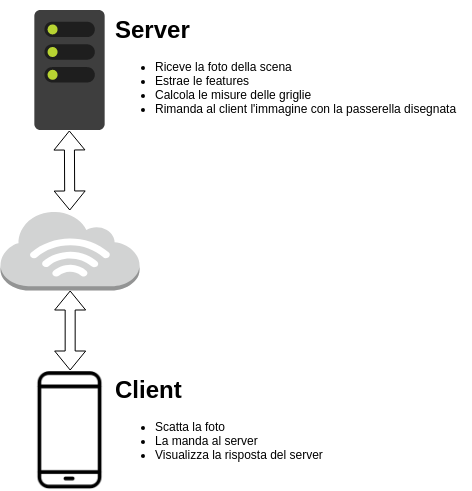
\includegraphics[scale=0.6]{images/Architettura.png}
  \caption{Architettura client-server}
\end{figure}
Descrizione dell'architettura software richiesta.
\section{Tecnologie utilizzate}
\subsection{Hardware}
\subsubsection{PC per lo sviluppo}
Portatile con Windows 10 Pro 64-bit:
\begin{figure}[H]
  \center
  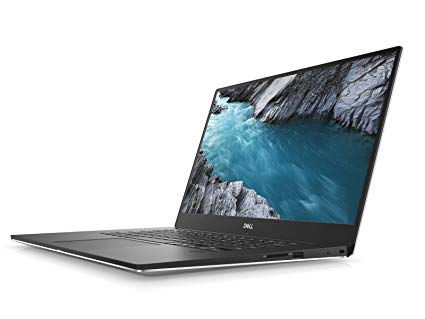
\includegraphics[scale=0.4]{images/pc.jpg}
  \caption{Dell XPS 9570}
\end{figure}
\begin{itemize}
  \item Intel Core i7-8750H CPU 2.20GHz x 12
  \item 16 GB 2 x 8 GB DDR4 a 2.666 MHz
  \item PCIe M.2 2280 da 512 GB
  \item NVIDIA GeForce GTX 1050 Ti con 4 GB di GDDR5
\end{itemize}
\subsubsection{Smartphone per l'acquisizione delle immagini}
Smartphone Android con fotocamera tripla Leica:
\begin{figure}[H]
  \center
  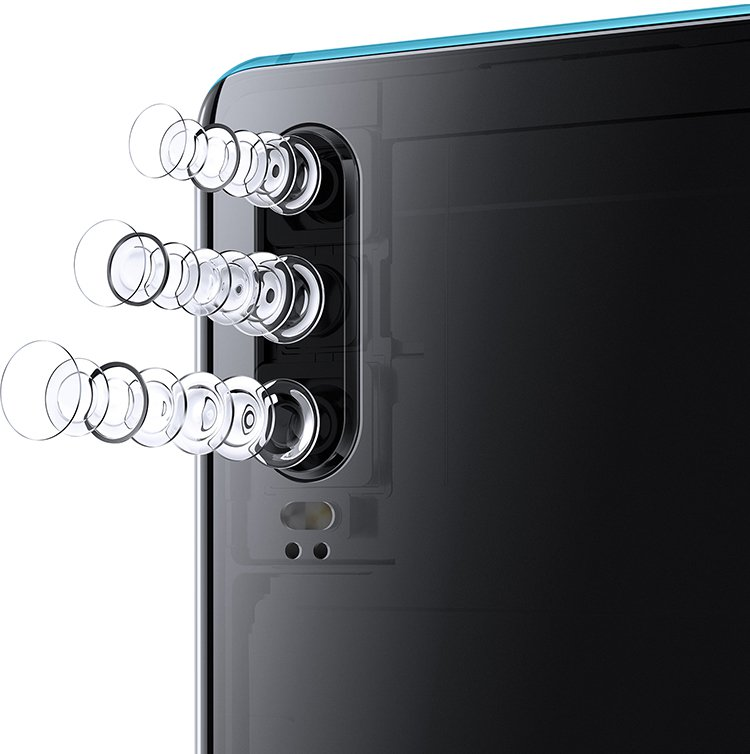
\includegraphics[scale=0.15]{images/smartphone.jpg}
  \caption{Huawei P30}
\end{figure}
\begin{itemize}
  \item 40 MP IMX650 Wide (f/1.8, 27mm, 1/1.7")
  \item 16 MP Ultrawide (f/2.2, 17mm)
  \item 8 MP Telephoto (f/2.4, 80mm, 1/4", OIS)
\end{itemize}
\subsection{Software}
\subsubsection{Ambienti di sviluppo, editor}
idea, pycharm, git, vscode.
\subsubsection{Elaborazione dell'immagine}
photoshop
\chapter{Diagrammi}

\section{Casi d'uso}
\begin{figure}[H]
  \center
  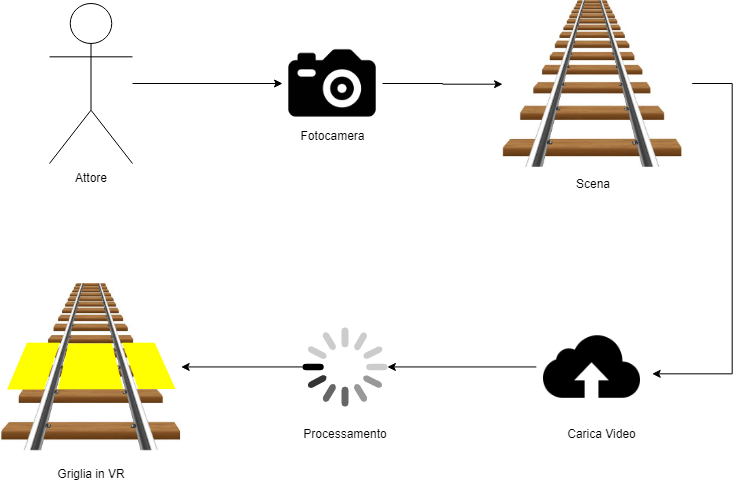
\includegraphics[scale=0.50]{images/UseCase.png}
  \caption{Diagramma}
\end{figure}
diagramma e relativa descrizione
\section{Sequenza}
\begin{figure}[H]
  \center
  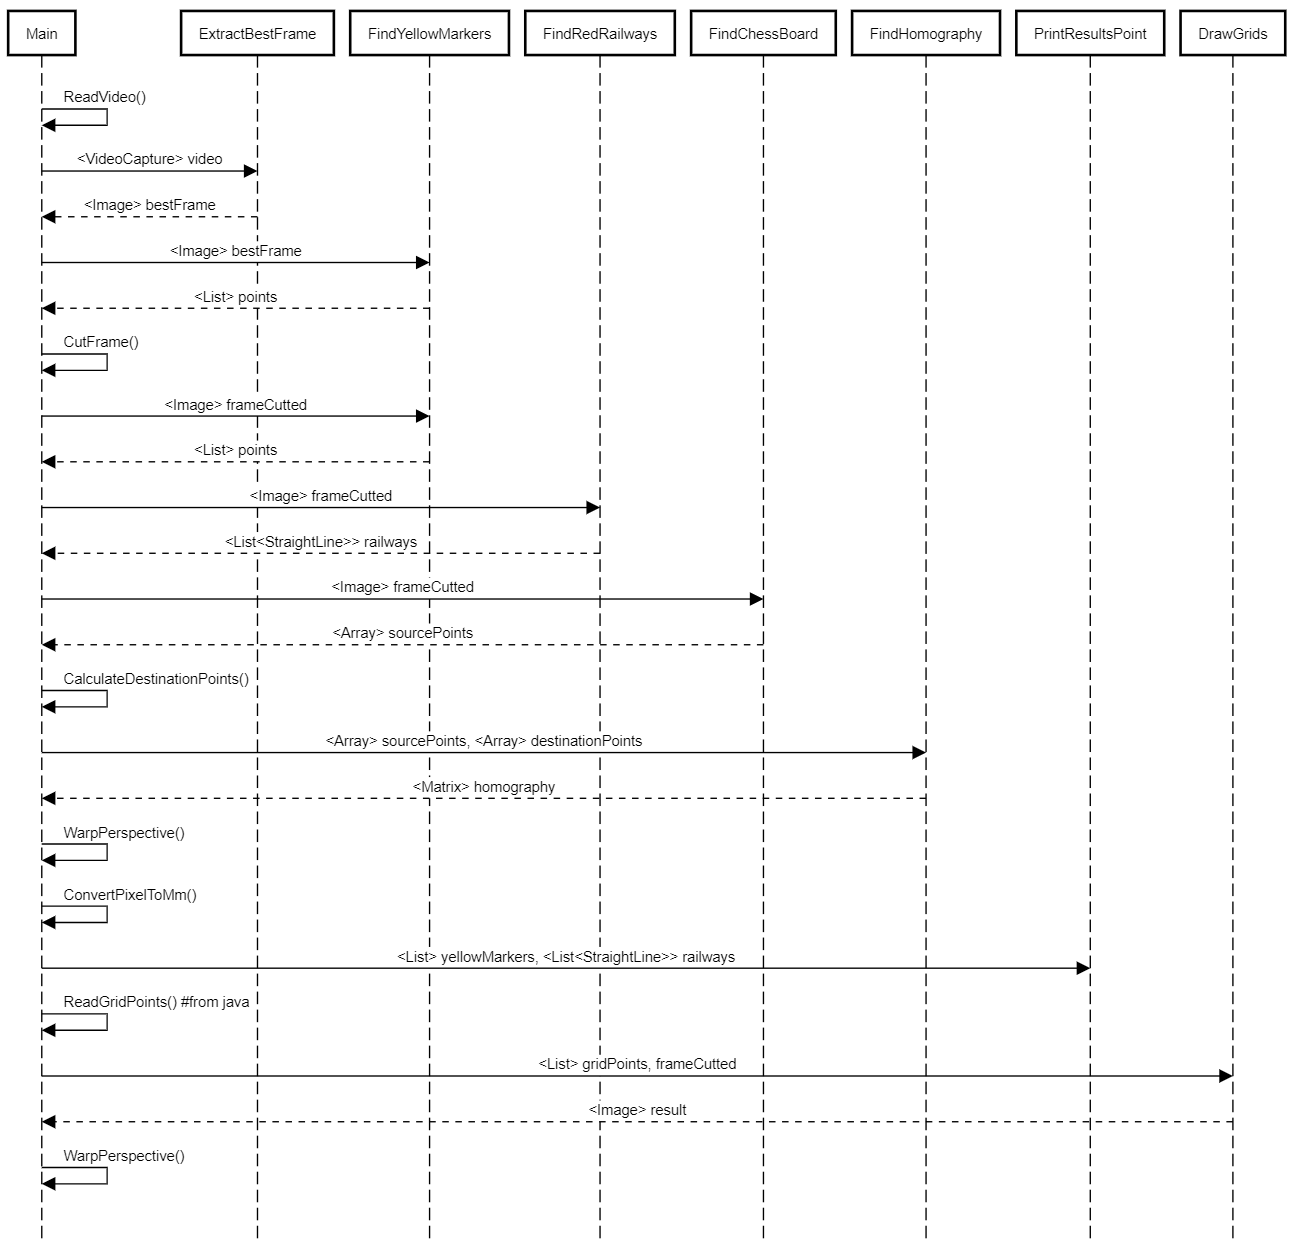
\includegraphics[scale=0.32]{images/Sequence.png}
  \caption{Diagramma}
\end{figure}
diagramma e relativa descrizione
\chapter{Implementazione}
\section{Linguaggi, librerie, framework}
\subsection{Java}
Java è un linguaggio di programmazione ad alto livello, orientato agli 
oggetti e a tipizzazione statica, che si appoggia sull'omonima piattaforma software, 
specificamente progettato per essere il più possibile indipendente dalla piattaforma 
hardware di esecuzione (tramite compilazione in bytecode prima e interpretazione poi 
da parte di una JVM), sebbene questa caratteristica comporti prestazioni in termini 
di computazione inferiori a quelle di linguaggi direttamente compilati come C e C++ 
ovvero dunque perfettamente adattati alla piattaforma hardware.
Il back-end dell'intera piattaforma è stato sviluppato mediante l'uso di questo linguaggio e 
del framework Spring MVC.
\subsection{Python}
È un linguaggio multi-paradigma che ha tra i principali obiettivi dinamicità, semplicità
e flessibilità. Supporta il paradigma object oriented, la programmazione strutturata e 
molte caratteristiche di programmazione funzionale e riflessione. Le caratteristiche più 
immediatamente riconoscibili di Python sono le variabili non tipizzate e l'uso 
dell'indentazione per la definizione delle specifiche. Altre caratteristiche distintive 
sono l'overloading di operatori e funzioni tramite delegation, la presenza di un 
ricco assortimento di tipi e funzioni di base e librerie standard, sintassi avanzate 
quali slicing e list comprehension.
Abbiamo scelto di utilizzare questo linguaggio in quanto la nota libreria OpenCV, descritta in 
seguito, è completamente supportata e documentata. Difatti gli script in python si occupano 
principalmente del processamento delle immagini. 
\subsection{OpenCV}
Descrizione di che cos'è opencv
\section{Feature detection}
In computer vision, e nell'elaborazione digitale delle immagini, il concetto di rilevamento
di caratteristiche (feature detection) o riconoscimento di caratteristiche racchiude una 
serie di metodi per l'estrapolazione di informazioni da una immagine e per prendere 
decisioni locali sull'esistenza o meno di una caratteristica in quel determinato punto. 
Le caratteristiche risultanti saranno un sottoinsieme del dominio dell'immagine, spesso 
in forma di punti isolati, curve continue o regioni connesse.
Non esiste una definizione universale ed esatta di cosa costituisca una caratteristica 
dell'immagine (image feature), e la definizione esatta spesso dipende dal problema o dal 
tipo di applicazione. Le caratteristiche sono usate spesso come punto di partenza da molti 
algoritmi di computer vision.
Una proprietà desiderabile per un rilevatore di caratteristiche è la ripetibilità: 
la stessa caratteristica dovrebbe essere rilevata in due o più differenti immagini della stessa scena.
È un'operazione di elaborazione delle immagini di basso livello, che ed esamina ogni pixel. 
È la prima operazione che si fa su un'immagine. Se invece fa parte di un algoritmo, 
allora di solito esamina solamente la regione individuata.
\subsection{Primo Approccio}
\subsubsection{Trasformata di Hough}
In computer vision esistono innumerevoli tecniche per l'estrazione delle features. Una 
di queste è la trasformata di Hough, utilizzata per individuare linee all'interno di una 
immagine. Ideata nella sua forma base agli inizi degli anni '60 da Paul Hough, fu in 
seguito perfezionata in una forma generalizzata e resa popolare nel 1981 da Dana H. 
Ballard, docente di informatica dell'università del Texas.
La trasformata di Hough necessita di un passo di preprocessing finalizzato all'Edge 
Detection (es Canny Edge Detection). L'immagine così ottenuta sarà una immagine in bianco e nero
dove i pixel bianchi rappresentano gli Edge, ovvero i contorni dei soggetti 
rappresentati. L'obiettivo della trasformata di Hough è di identificare quali di questi 
contorni rappresentino una linea retta: se più pixel di Edge sono allineati, anche se non 
connessi tra loro, viene individuata una linea nell'immagine.
Per rappresentare una linea retta servono due parametri: un coefficiente angolare $m$ e 
una ordinata all'origine $c$. Considerato un singolo punto, questo appartiene a infinite 
rette della forma $y=mx+q$, al variare di $m$ e $q$. Dobbiamo quindi stabilire quali coppie 
$(m,q)$ siano in grado di individuare al meglio gli allineamenti di pixel.
L'idea della trasformata di Hough è di rappresentare le rette nello spazio parametrico 
$m-q$. In questo modo preso un punto $(x,y)$ l'equazione $y=mx+q$ andrà a rappresentare 
una sola retta invece di infinite. Nello spazio parametrico vengono quindi rappresentate 
tante rette quanti sono i pixel di edge. Se queste rette si intersecano, i due punti 
corrispondenti dell'immagine risulteranno allineati sulla retta con i coefficienti 
$(m,q)$ corrispondenti. La tecnica sembra quindi funzionare: le rette corrispondenti ad 
un alto numero di intersezioni nello spazio parametrico sono le linee che volevamo 
ottenere.
\begin{figure}[H]
  \center
  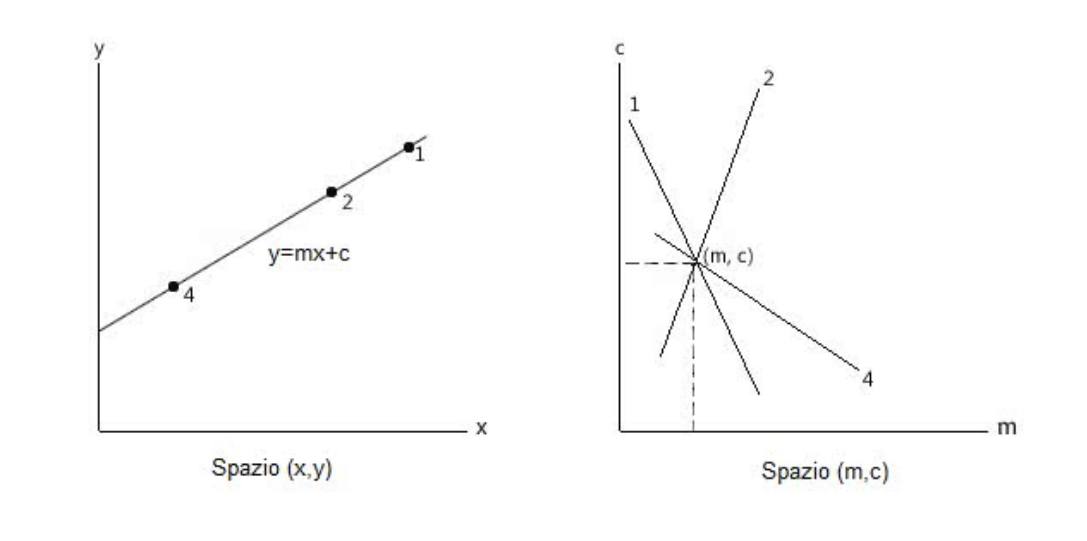
\includegraphics[scale=0.38]{images/spazioMC.png}
  \caption{I parametri m e q vengono mappati nello spazio parametrico e la linea è 
  individuata dall'intersezione delle rette.}
\end{figure}

La trasformata però in questa forma presenta dei problemi che non la rendono applicabile 
su un calcolatore. Infatti per linee verticali il coefficiente angolare $m$ tende all'infinito, 
contrastando le limitazioni di memoria di ogni computer. Si ricorre quindi ad una versione 
detta forma normale dove le rette vengono rappresentate mediante la forma $xcos\theta+ysin\theta=r$.
I parametri $\theta$ e $r$ sono rispettivamente l'angolo e la distanza della retta dall'origine. 
Quantizzando $\theta$ e utilizzando come spazio parametrico $\theta-r$ si risolve quindi il problema 
della finitezza della memoria.
All'interno della libreria OpenCV la traformata di Hough si ottiene tramite la funzione:
\begin{lstlisting}[language=Python]
def HoughLinesP(image, rho, theta, threshold, lines=None, 
                minLineLength=None, maxLineGap=None):
\end{lstlisting}
\begin{itemize}
  \item \textbf{image:} puntatore all'immagine degli edge ottenuta tramite un algoritmo di 
  Edge Detection.
  \item \textbf{rho:} spessore in pixel delle linee rappresentate nello spazio parametrico. 
  Viene utilizzato per accorpare tra loro intersezioni vicine.
  \item \textbf{threshold:} soglia sul numero di intersezioni che si devono ottenere 
  affinchè una linea sia identificata come tale.
  \item \textbf{lines:} struttura dove la funzione scrive le linee, tipicamente sotto forma 
  di CvMemoryStorage.
  \item \textbf{minLineLength:} rappresenta la lunghezza minima di una linea.
  \item \textbf{maxLineGap:} rappresenta a distanza tra punti sulla stessa retta, per 
  spezzarla in due linee differenti.
\end{itemize}
\subsubsection{Binari}
\begin{figure}[H]
  \center
  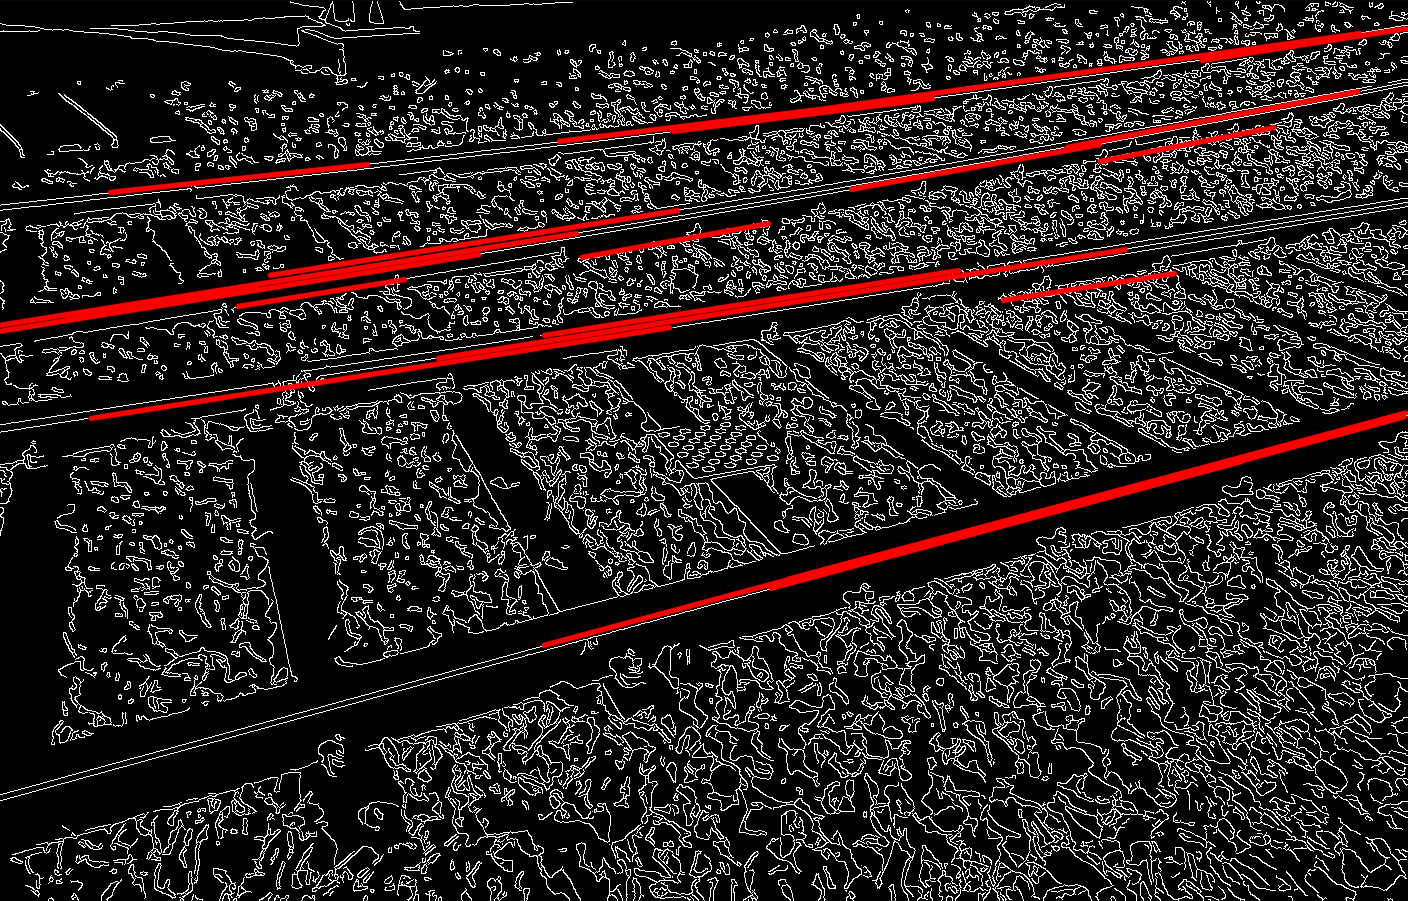
\includegraphics[scale=0.25]{images/houghLines.png}
  \caption{Ricerca dei binari mediante la trasformata di Hough}
\end{figure}
Come si evince dall'immagine sopra, mediante la trasformata di Hough è possibile identificare 
i binari all'interno di una foto. Al fine di identificare solo i binari e non altre linee rette
è necessario settare correttamente i parametri, in particolar modo il valore di threshold e 
la lunghezza minima delle rette. Per torvare il valore ottimale di threshold abbiamo usato la soglia OTSU 
calcolata sfruttanto la varianza tra classi di pixel (l'algoritmo che calcola questa soglia è implementato nativamente
nella libreria OpenCV). Invece per determinare la lunghezza minima delle linee abbiamo effettuato un calcolo 
assumendo che un binario sia lungo quanto la larghezza o lunghezza della foto. Tuttavia, si può notare
come un binario può essere identificato da più rette. Inoltre, nonostante il settaggio corretto dei parametri 
è comunque possibile che vengano rilevate linee che non centrano nulla con i binari. L'approccio scelto
per risolvere questi due problemi è di tipo matematico. Per identificare un binario con una sola abbiamo deciso di raggupparle
sfruttando l'area sottesa alla retta trovata, ovvero l'integrale, assumendo che due rette che rappresentano lo stesso binario 
hanno un'area circa uguale. Infine per identificare solo i binari e non altre linee rette abbiamo rimosso 
tutte le rette che si intersecano all'interno dello spazio definito dalla foto e per maggiore sicurezza l'immagine è anche stata 
sfocata mediante un filtro gaussiano al fine di far rimanere in evidenza solo le linee dei binari.
\begin{figure}[H]
  \center
  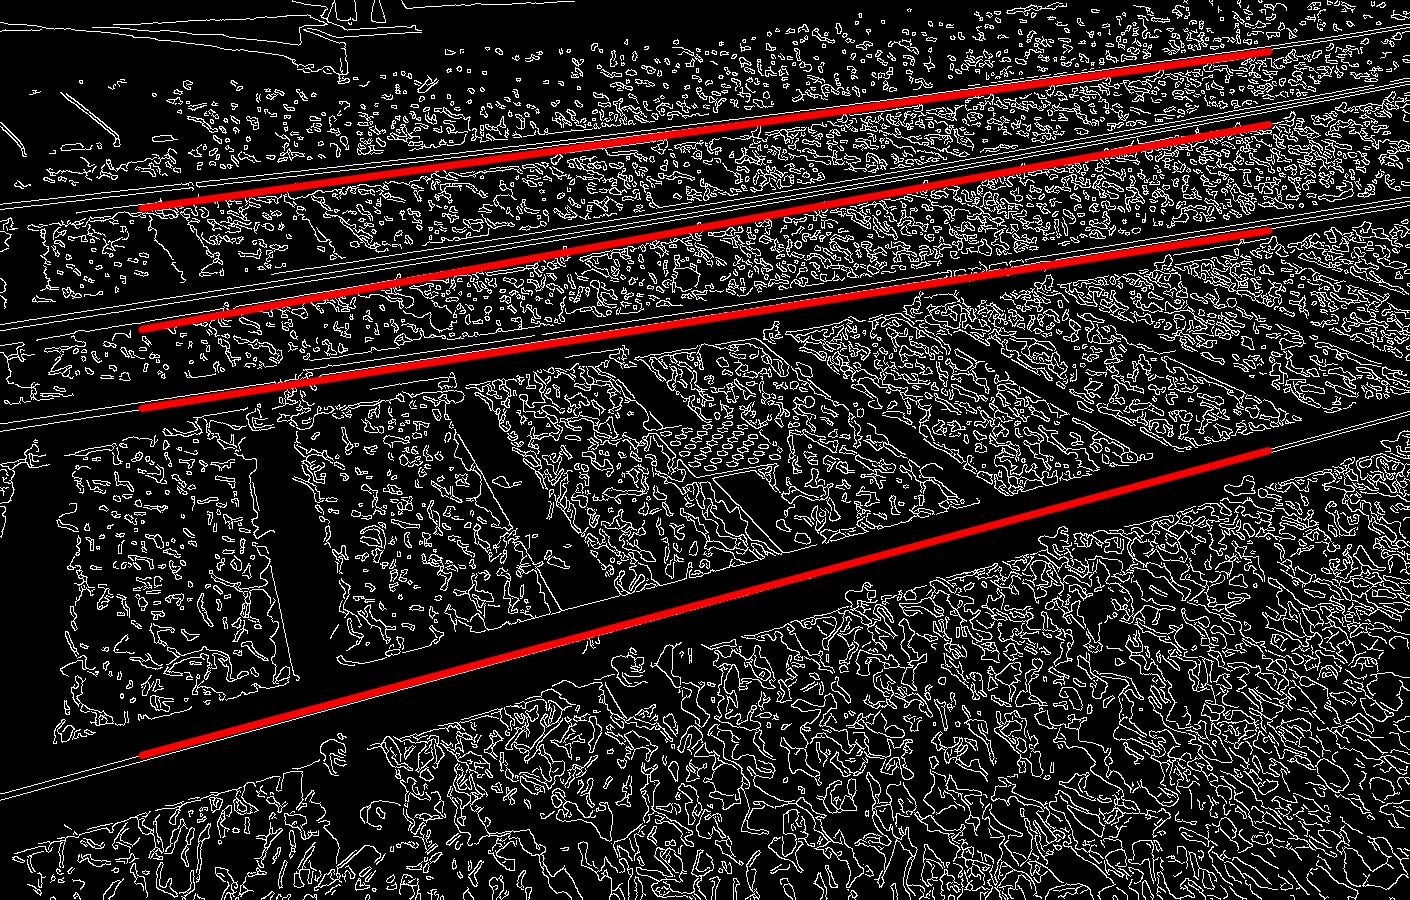
\includegraphics[scale=0.25]{images/houghLinesMerged.jpg}
  \caption{Risultato filtraggi matematici}
\end{figure}
Il risultato ottenuto sembra promettere bene tuttavia, sfruttando questa tecnica si rischia di non fare distinzione tra 
il lato interno o esterno del binario. Inoltre non è possibile determinare se la linea identifica il binari sullo stesso piano. 
Come soluzione abbiamo deciso di sfruttare i bulloni delle traversine messe in risalto con del nastro rosso. Posizionandone anche solo 
quattro è possibile identificare correttamente i binari. 
\subsubsection{Punti}
\begin{figure}[H]
  \center
  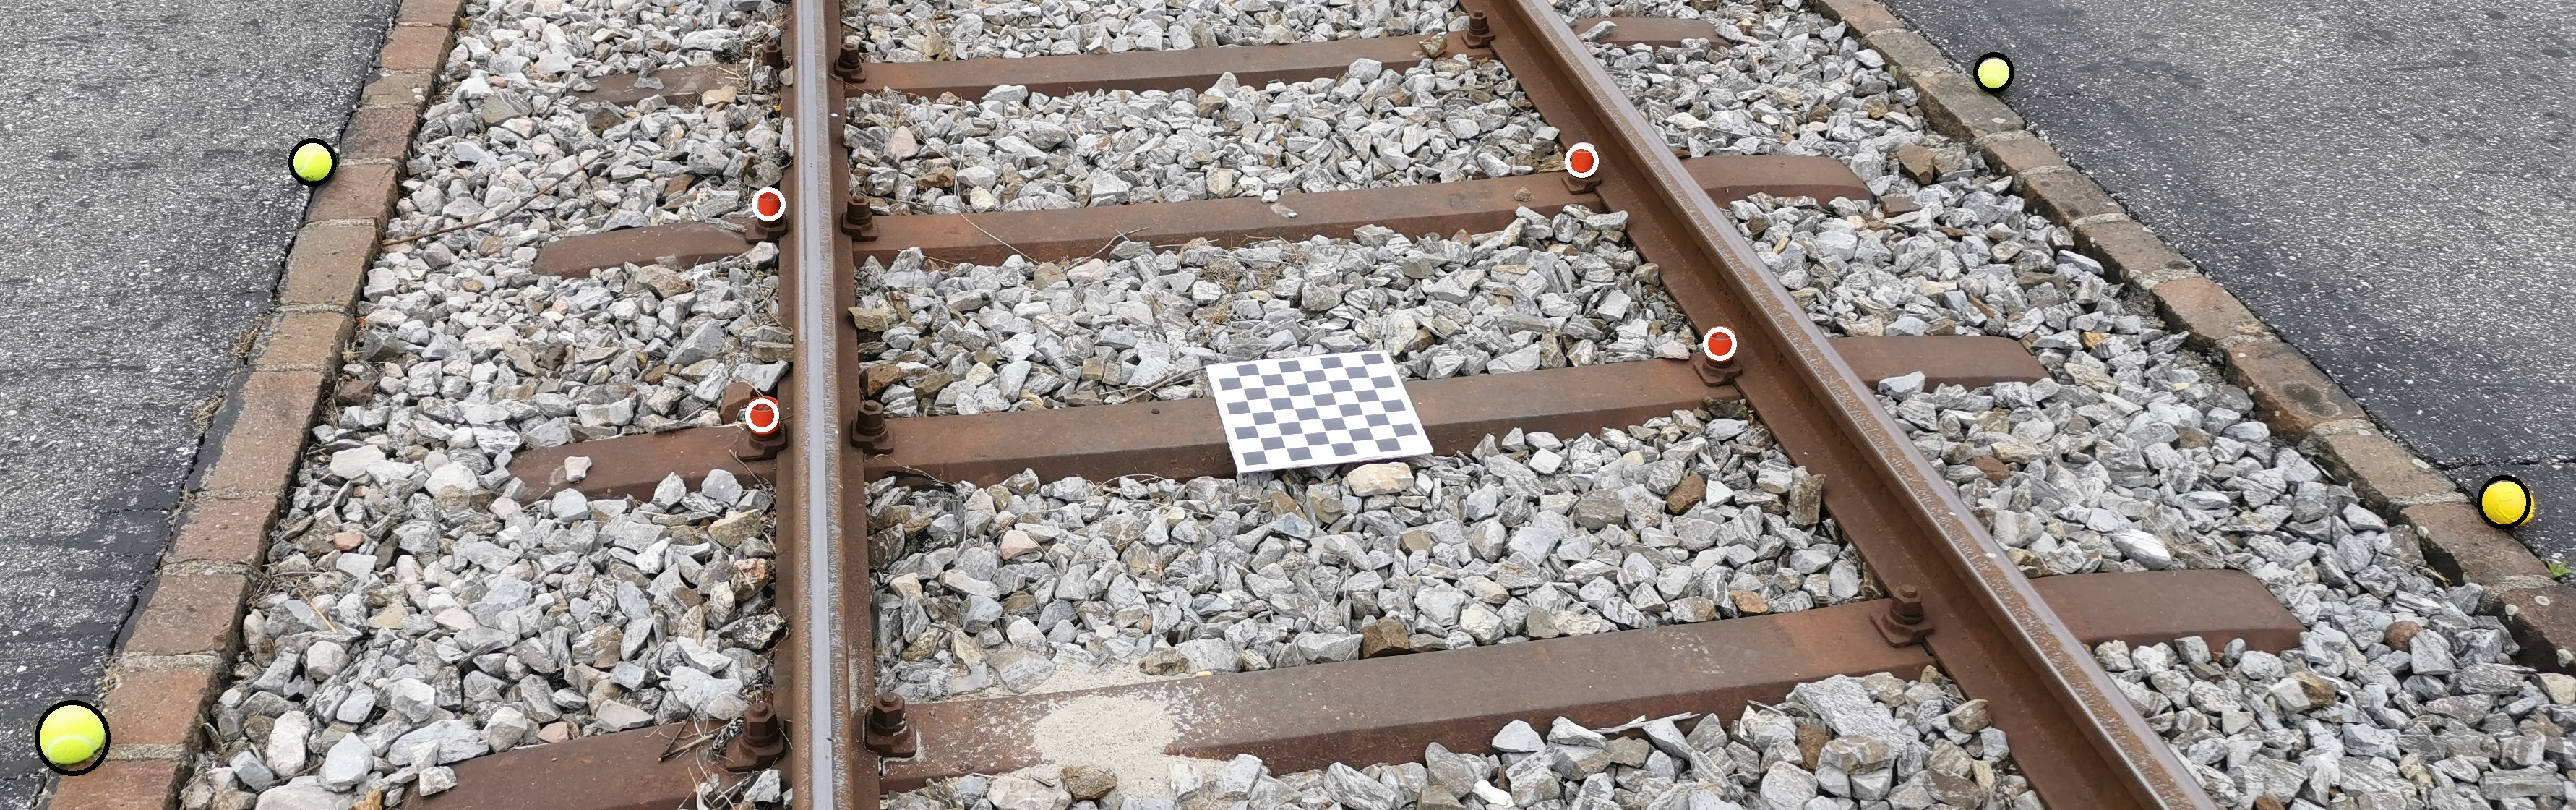
\includegraphics[scale=0.08]{images/points.jpg}
  \caption{Rilevamento delle palline da tennis e dei nastri rossi}
\end{figure}
Per il rilevamento dei punti abbiamo sfruttato due diversi approci a seconda del tipo di punto da rilevare. Nonostante questo il punto di 
partenza delle tecniche è il medesimo: il colore. Abbiamo effettuato un filtraggio sul colore in modo da avere il resto dell'immagine
nera e solo i punti di nostro interesse in risalto. 
\begin{figure}[H]
  \center
  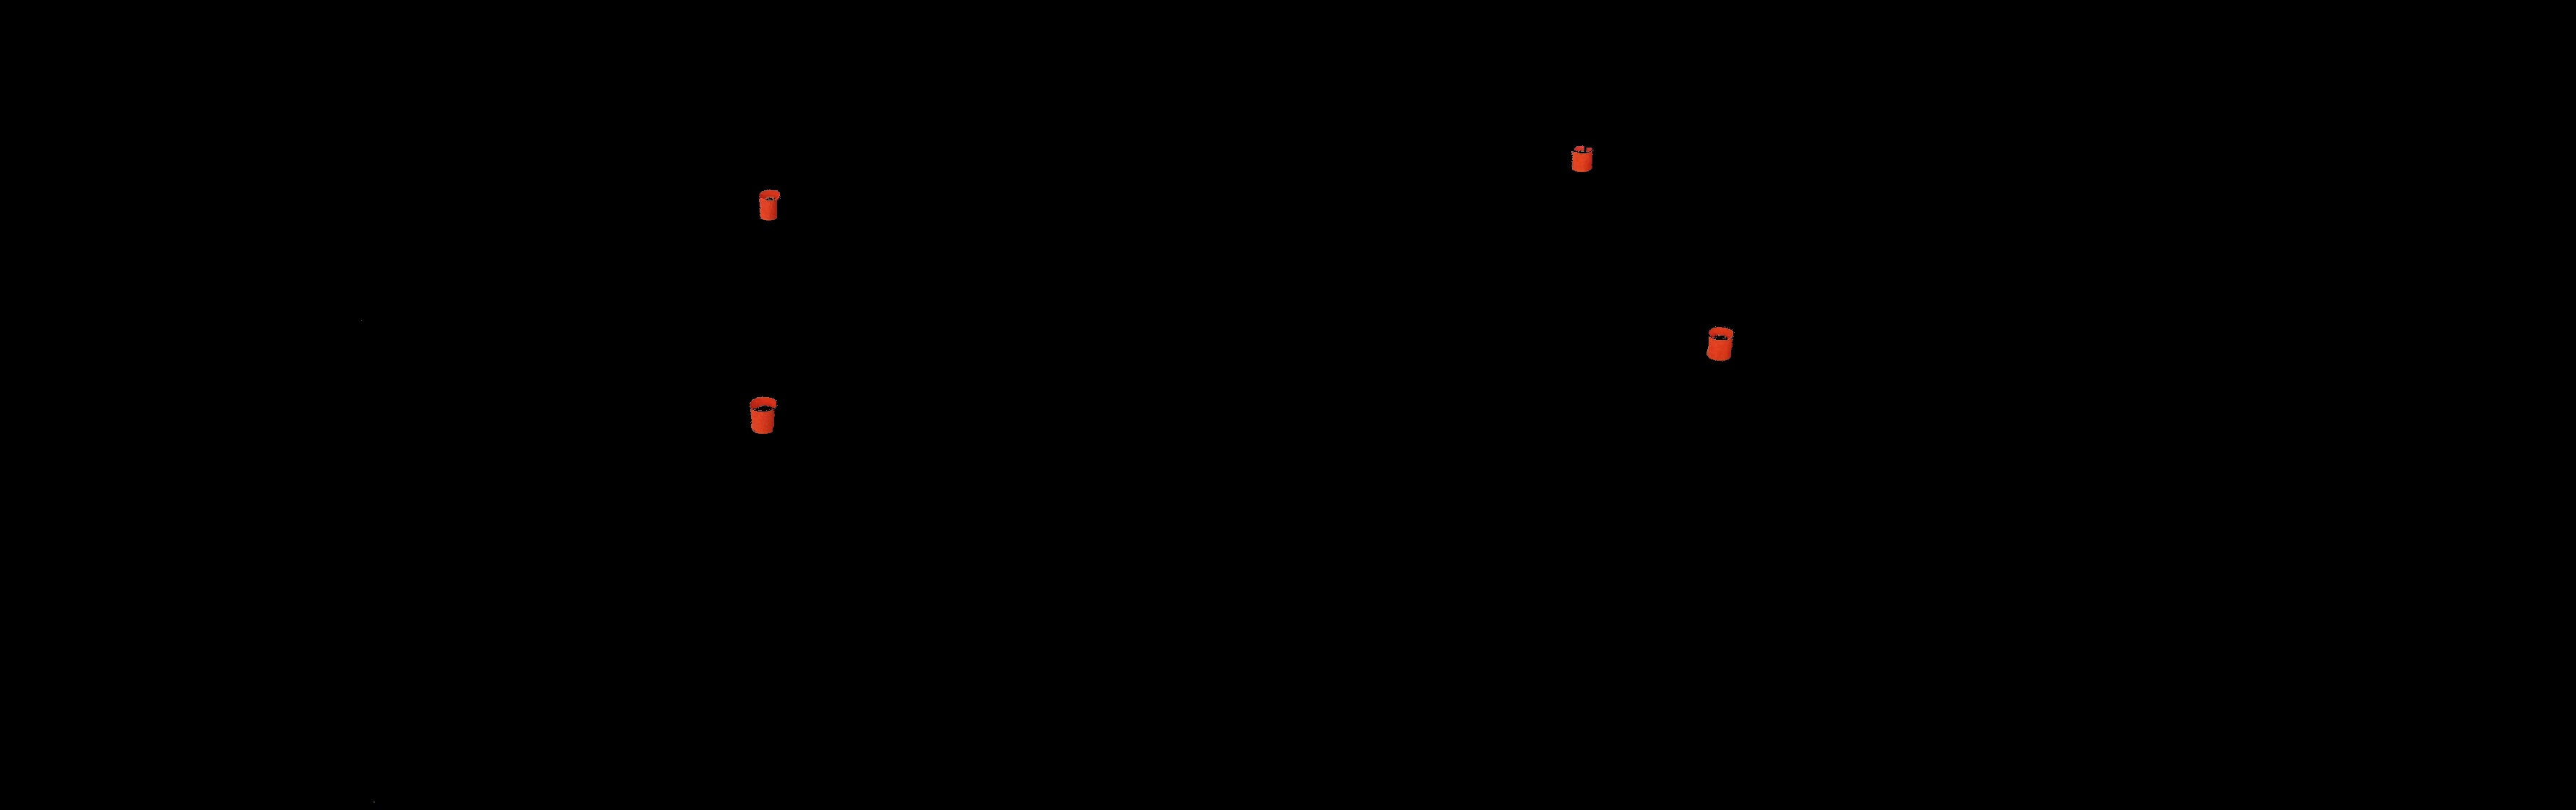
\includegraphics[scale=0.08]{images/points1.jpg}
  \caption{Filtraggio sul colore del nastro rosso}
\end{figure}
Nell'immagine sopra sono rimasti solo i nastri rossi, in questo modo ci è stato possibile ricercare i contorni delle regioni di colore rosso e 
identificare così i 4 bulloni. Nel caso delle palline da tennis abbiamo risfruttato l'algoritmo di Hough mediante la seguente funzione:

\begin{lstlisting}[language=Python]
def HoughCircles(image, method, dp, minDist, circles=None, 
                 param1=None, param2=None, minRadius=None, 
                 maxRadius=None):
\end{lstlisting}
\begin{itemize}
  \item \textbf{image:} puntatore all'immagine degli edge ottenuta tramite un algoritmo di 
  Edge Detection.
  \item \textbf{method:} metodo sfruttato per il rilevamento di circonferenze, 
  l'unico attualmnete disponibile e quello del gradiente.
  \item \textbf{dp:} rapporto inverso della risoluzione (default 1).
  \item \textbf{minDist:} distanza minima tra il centro delle circonferenze rilevate.
  \item \textbf{circles:} array di output.
  \item \textbf{param1:} soglia superiore per il processo di edge detection (Canny).
  \item \textbf{param2:} soglia per il rilevamento del centro, più è bassa più si 
  rischiano falsi positivi.
  \item \textbf{minRadius:} raggio minimo delle circonferenze da rilevare.
  \item \textbf{maxRadius:} raggio massimo delle circonferenze da rilevare.
\end{itemize}

\subsection{Secondo approccio}
\subsubsection{Shape detection}
descrizione di come vengono rilevati gli oggetti mediante il loro colore e i contorni
\subsubsection{Binari}

\subsubsection{Punti}

\subsection{Foto o video}

\subsection{Approccio scelto}
spiega perchè si è utilizzata la shape detection e perchè si è scelto di introdurre un video della scena.

\section{Calibratore}
descrizione di che cos'è e di come si usa

\section{Matrice Omografica}
In matematica e geometria una omografia è una relazione tra punti di due spazi tali per cui ogni punto di uno spazio corrisponde ad uno ed un solo
punto del secondo spazio. In Computer Vison il concetto alla base è circa lo stesso: definiamo l'omografia planare come una “mappatura proiettiva” da
una superficie per un’altra. L’esempio più classico di omografia, che viene usato da ognuno di noi quotidianamente, è sicuramente la mappatura dei
punti su una superficie planare bidimensionale fatta dal sensore della nostra macchina fotografica. È possibile esprimere questa mappatura come
moltiplicazione di matrici. Sfruttando le coordinate omogenee definiamo un punto nella realtà $\vec{Q}$ e la sua “mappatura” $\vec{q}$ effettuata dal sensore:
\begin{align}
  \vec{Q} &= \begin{bmatrix}
         X \\
         Y \\
         Z \\
         1
       \end{bmatrix}, and 
       \vec{Q} &= \begin{bmatrix}
        X \\
        Y \\
        Z \\
        1
      \end{bmatrix}
\end{align}
\section{Interfacciamento sistema pre esistente}
breve descrizione progetto biella perrone 

\section{Gestione errori}
descrizione dei controlli effettuati durante il processamento delle immagini

\section{Testing e risultati ottenuti}
esempio d utilizzo con confronto tra le misure reali e quelle ottenute

\chapter{Conclusioni}
analisi dei risultati ottenuti 

\section{Problematiche}
- scelta dell'approccio corretto
- matematica e algebra
- misure su piani differenti

\section{Sviluppi futuri}
\subsection{Utilizzo della focale}
\begin{figure}[H]
  \center
  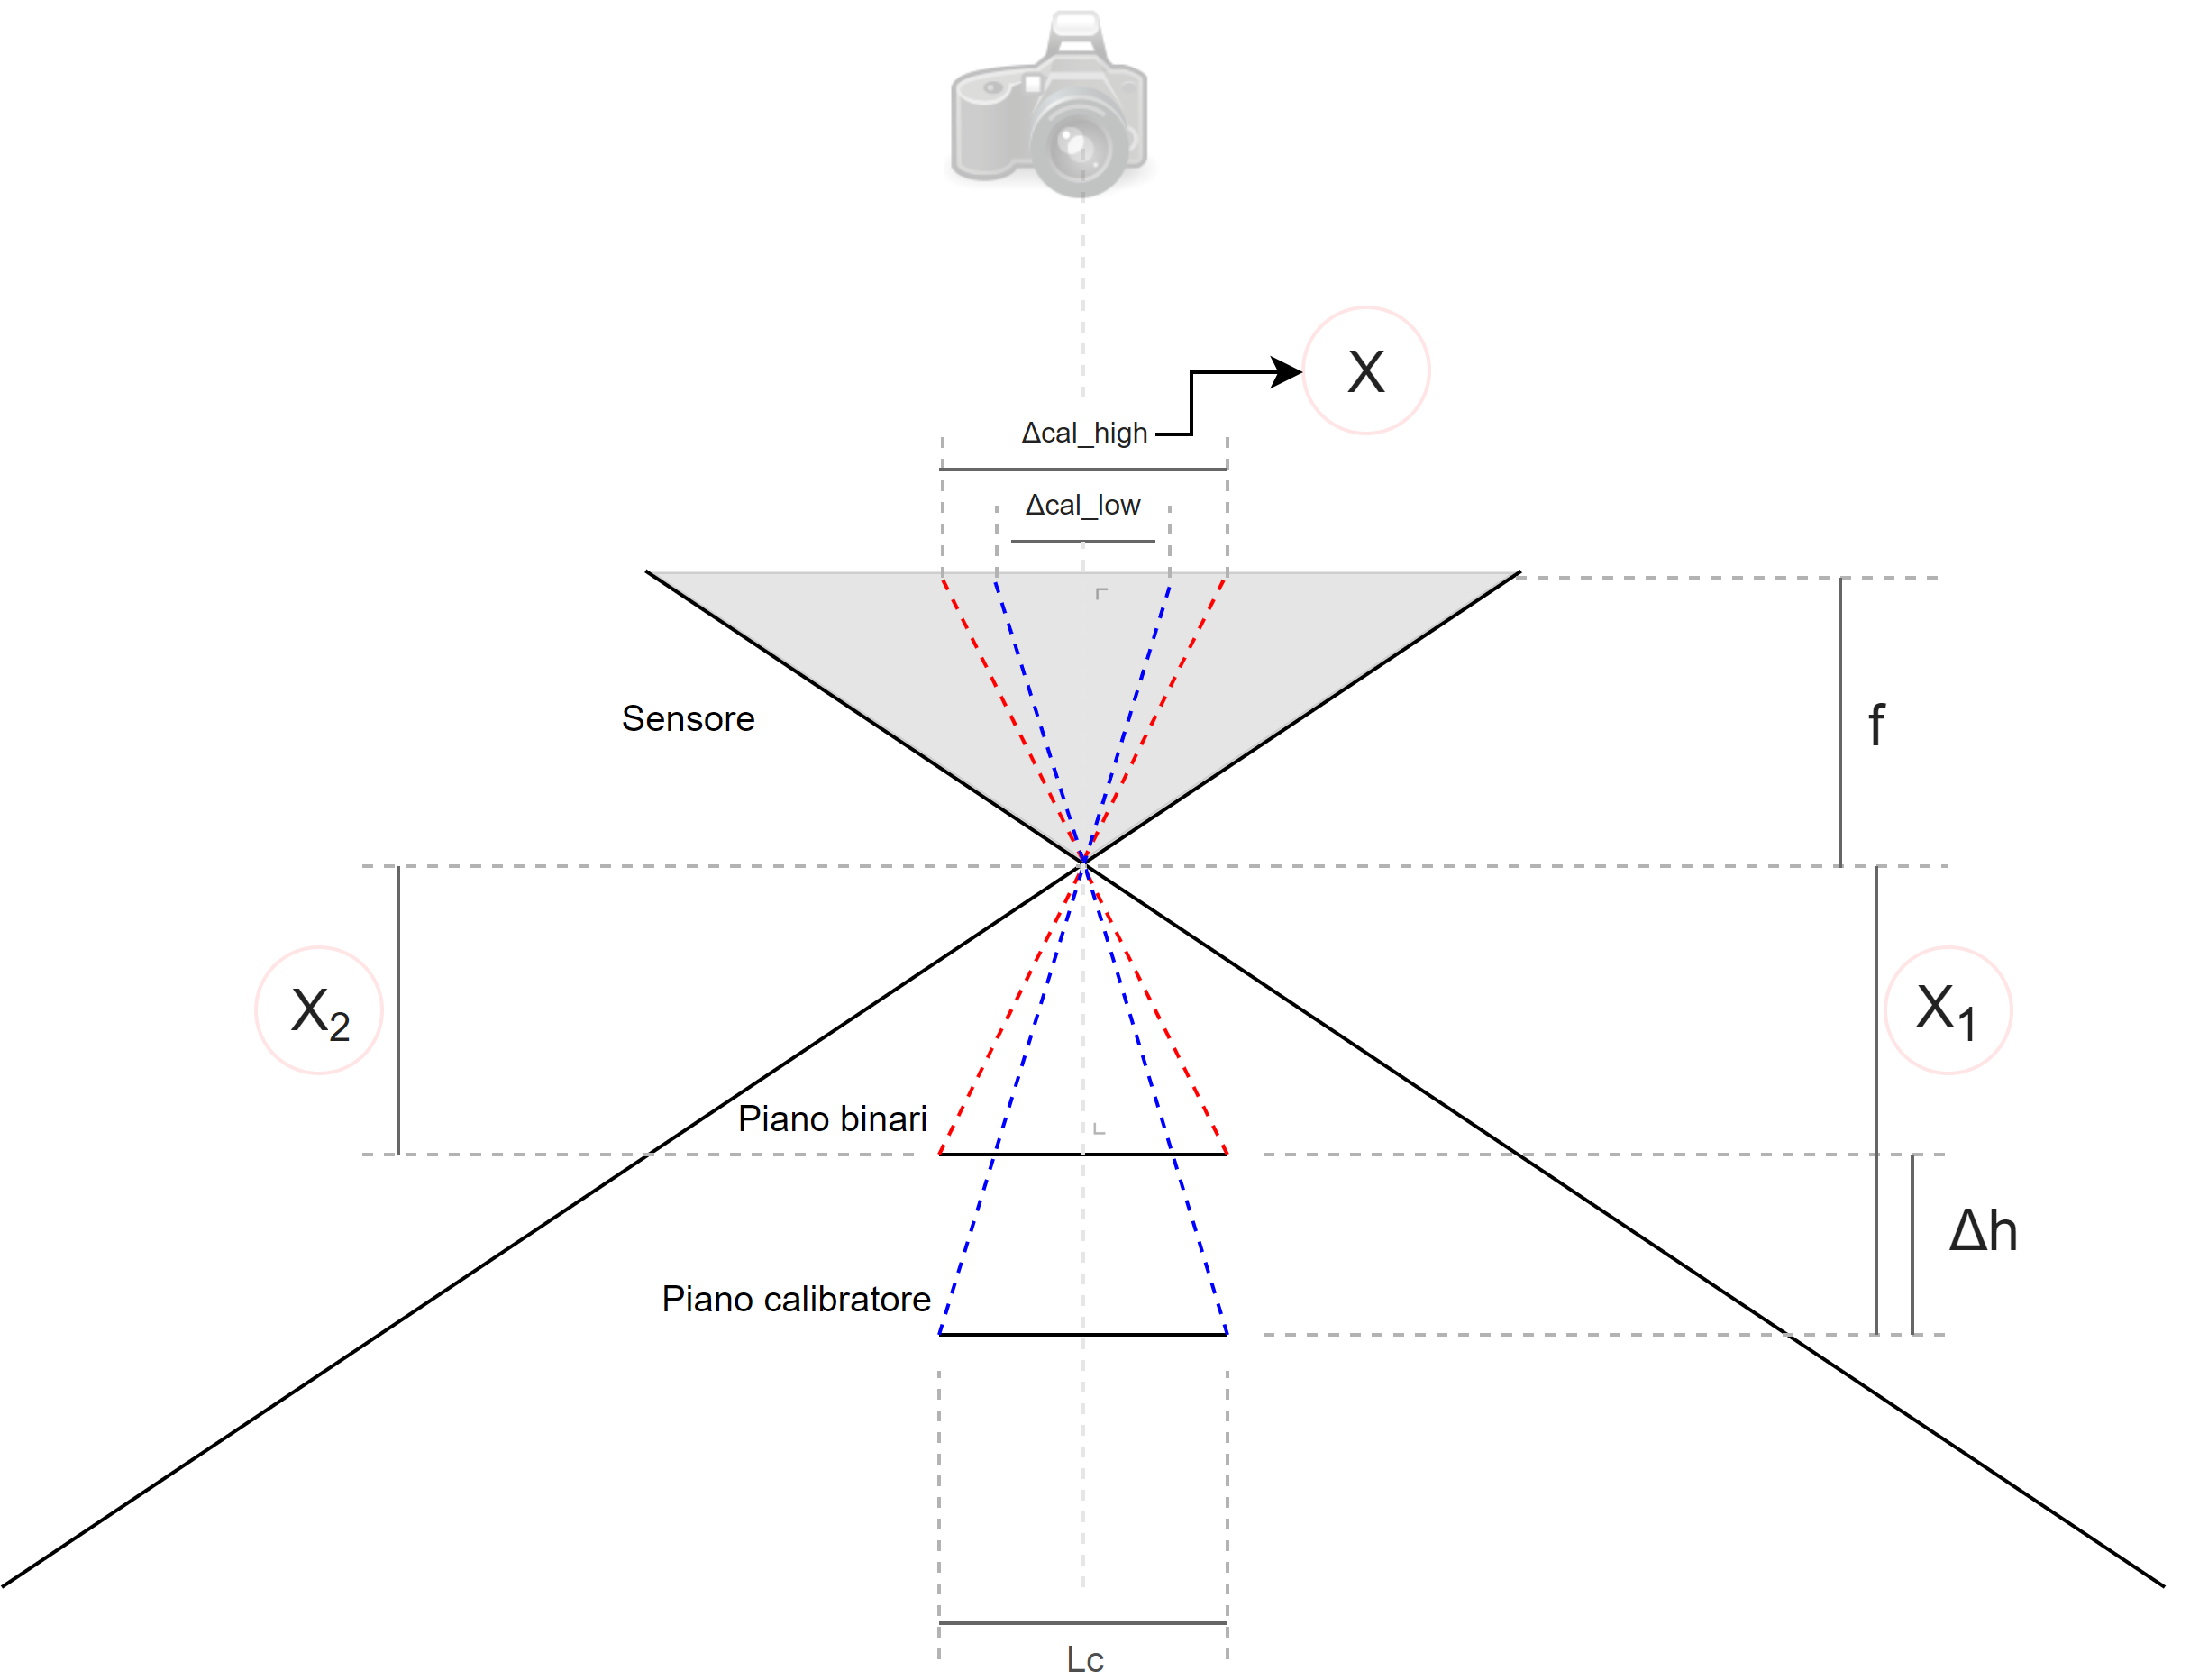
\includegraphics[scale=0.45]{images/ProblemaAltezza.png}
  \caption{Disegno esplicativo della focale}
\end{figure}
\subsection{Calibrazione della camera}
\subsection{Concatenazione di più fotografie}
\subsection{Controllo online della ripresa video}

\section{Considerazioni finali}
cosa mi è piaciuto in particolare del progetto, soddisfazione etc.

\bibliographystyle{unsrt}\nocite{*}
\bibliography{bibliografia}
\end{document}
